%%% EtherPad for Discrete Mathematics VO
%%% http://www.informatik-forum.at/showthread.php?104454-Notes-2013WS-VO_01
%%% Past pads:
%%%     * 2013-10-17: committed by patrikf
%%%     * 2013-10-18: committed by patrikf
%%%     * 2013-10-24: committed by patrikf
%%%     * 2013-10-25: committed by patrikf
%%%     * 2013-11-08: committed by neroburner
%%%     * 2013-11-21: committed by neroburner
%%%     * 2013-11-22: committed by neroburner

% Discrete Mathematics Lecture Notes 2013-11-28
% raw data written by only neroburner...

\textbf{Repetition of last time.}
\lecturedate[\baselineskip]{2013-11-28}
labelled structure set $\mathcal{A} = (A,w)$, the atomic object can be enumerated.

\begin{align*}
  \mathcal{A}+\mathcal{B} &\leftrightarrow \hat{A}(z) + \hat{B}(z) \\
  \mathcal{A}*\mathcal{B} &\leftrightarrow \hat{A}(z) * \hat{B}(z) \\
  \seq(\mathcal{A}) &\leftrightarrow \frac{1}{1 - \hat{A}(z)}\\
  \set(\mathcal{A}) &\leftrightarrow \exp(\hat{A}(z)) \\
  \cyc(\mathcal{A}) &\leftrightarrow \log \frac{1}{1 - \hat{A}(z)}\\
\end{align*}

% end of repetition

\textbf{Example.}
\begin{align*}
  \mathcal{P} &= set(cyc(\mathcal{A})), \mathcal{A} = \{ \text{\ding{172}} \}\\
  \hat{P}(z)  &= \exp{(\log{\frac{1}{1-z}})} = ∑_{n≥0} n! \frac{z^n}{n!}
\end{align*}

\textbf{Example.}
we got set partitions $M = M_1 \cup M_2 \cup \ldots \cup M_k$ with $M_i \neq \varnothing$ and $M_i \cap M_j = \varnothing$
\begin{align*}
  \mathcal{P} = \set( \set( \mathcal{A}) \backslash \{\varnothing\} ) \\
  \hat{P}(z) = \exp(\exp((z) - 1) \\
  [z^n] e^{e^z - 1} = \sum_{k\geq 0 } S_{n,k} \\
\end{align*}

\subsection{Exponential Generating Functions and Ordered Structures}

Ordered n-tuples $(q_1,q_2, \ldots, q_n), q_i \in \{1,2, \ldots, N\}$, no repetition

$a_n$ is number of such n-tuples

$Q = \underbrace{\{\epsilon,1\}}_{1+z} *
     \underbrace{\{\epsilon,2\}}_{1+z} * \ldots *
     \underbrace{\{\epsilon,N\}}_{1+z} $

\begin{align*}
  \sum_{n\geq 0} a_n \frac{z^n}{n!} &=
    (1+z)^N \\
    &= \sum_{n=0} ^{N} {N \choose n} z^n \\
    &= \frac{N!}{(N-n)!}
\end{align*}

With repetition:
\[
  (1+z+ \frac{z^2}{2!} + \frac{z^3}{3!} + \ldots)^N
    = e^{zN} = \sum_{n\geq 0} N^n \frac{z^n}{n!}
\]

\section{Combinatorics on posets}

Recall $(A, \leq) \subseteq A \times A$.
Instead of $(a,b) \in \, \leq$ we use the notation $a \leq b$. So $\leq$ is a partial order.

\begin{tabular}{ll}
  1) $\leq$ reflexive: &
    $\forall x \in A: x \leq x$ \\
  2) $\leq$ transitive:  &
    $\forall x,y,z \in A: x \leq y \land y \leq z \implies x \leq z$ \\
  3) $\leq$ antisymmetric: &
    if $x \leq y \land y \leq x$ then $x = y$ \\
\end{tabular}

$(A,\leq)$ is a poset.

A poset $(A,\leq)$ is linearly ordered if
\[
  \forall x,y, \in A: x \leq y \lor y \leq x
\]

\textbf{Examples.}\\\\
\begin{tabular}{l l}
  $(\mathbb{N}, \leq), (\mathbb{R}, \leq)$: & Posets, even linearly ordered \\\\

  $(\mathbb{N}^{+}, |)$:
    & $a|a$ \\
    & $ a|b, b|c \implies a|c$\\
    & $ a|b \land b|a \implies a = b$\\
    & Poset, not linearly ordered since $2 \not|~ 3 \land 3 \not|~ 2$\\\\

  $(2^A, \subseteq)$:
    & $ B \subseteq B$\\
    & $ B \subseteq C \subseteq D$\\
    & $ B \subseteq C \land C \subseteq B \implies B = C$ \\
    & Poset, If $|A|\leq 1$ then it is even a linear ordered poset.
\end{tabular}

\begin{definition}
Given a poset $(A, \leq)$.
An element $x \in A$ is a \dt{minimal element} if $y \leq x \implies x=y$.
Each poset can be visualized by a Hasse diagram

\begin{center}
    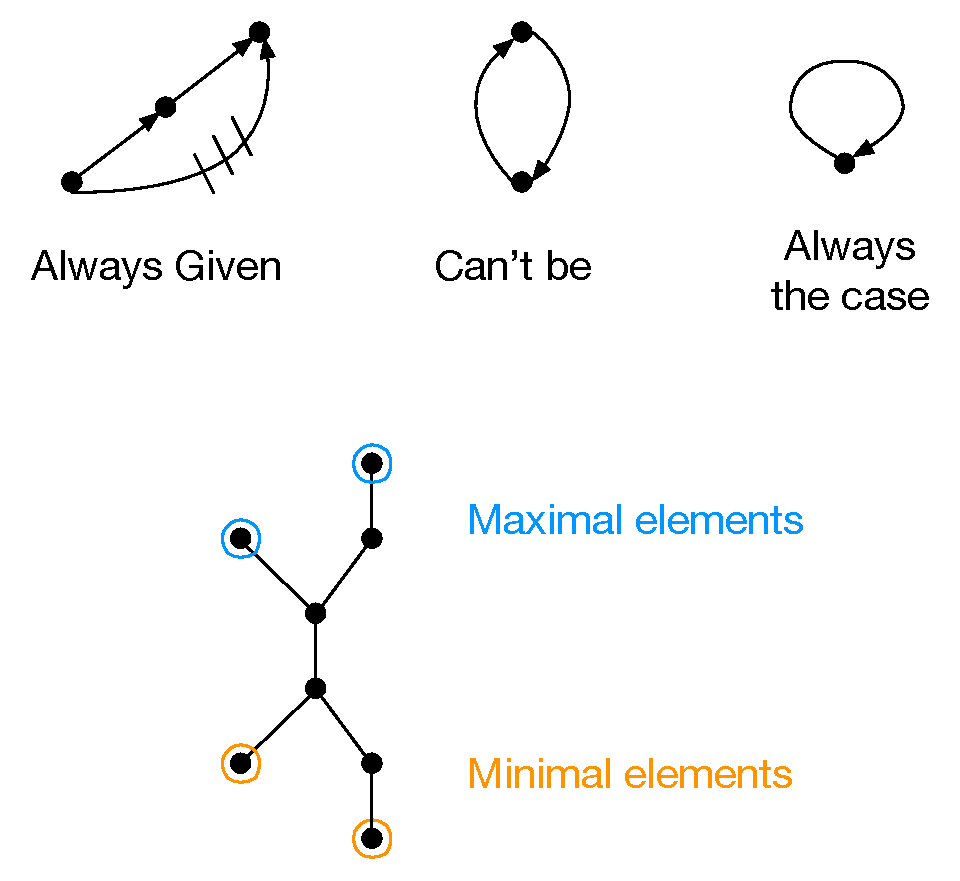
\includegraphics[width=0.6\textwidth]{02_higher_combinatorics/pics/Lattice}
\end{center}

An element $x \in A$ is
\begin{compactitem}
  \item a \dt{maximal element} if $y \geq x \implies x=y$
  \item the \dt{0-element} if $\forall y \in A : x \leq y$ \\
    (every 0-element is minimal)
  \item the \dt{1-element} if $\forall y \in A : x \geq y$
\end{compactitem}~\\
Interval $[x,y] = \{z \in A \mid x \leq z \leq y\}$

$(A, \leq)$ is locally finite if $\forall x,y \in A: | [x,y]| < \infty$.
\end{definition}

\textbf{Examples.} \\
\begin{tabular}{ll}
  $(\mathbb{N}, \leq)$
    & 0, $\nexists$ 1-element, locally finite \\
  $(\mathbb{N}^{+}, \mid)$
    & locally finite, 0-element = $1$ \\
  $(\mathbb{N}, \mid)$,
    & 1-element = $0$ \\
  $(\mathbb{R}, \leq)$
    & not locally finite
\end{tabular}

\textbf{Assumptions.}
Let $(\mathbb{P}, \leq)$ be a locally finite poset. And we have a map $f \rightarrow \mathbb{R}$, and some function $S_f(x) = \sum_{z \leq x} f(z)$

\textbf{Example.}

\begin{tabular}{ll}
  1) & \\
     & $(\mathbb{N}, \leq)$\\
     & $f \leftrightarrow (a_n)$\\
     & $S_f \leftrightarrow \sum_{k\leq n} a_k$\\\\

  2) & \\
     & 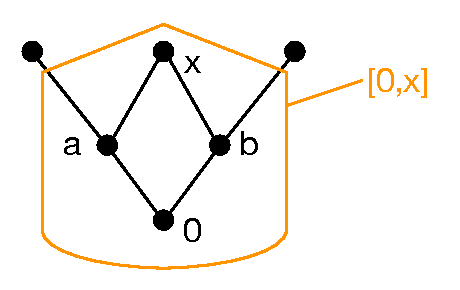
\includegraphics[width=0.4\textwidth]
        {02_higher_combinatorics/pics/LatticeInterval}\\
     & $S_f(x) = f(0) + f(a) + f(b) + f(x) $\\
     & $a_n = \sum_{k \leq n} a_k - \sum_{k \leq n-1} a_k =
              S_f(n) - S_f(n-1)$\\
\end{tabular}~\\

\textbf{Problem.}
Given $S_f$, find $f$

\begin{definition}
$(P, \leq)$ is a locally finite poset with a 0-element.
We have a \dt{Möbius function} of $P$ $\mu: P\times P \rightarrow \mathbb{R}$.
if
\[
  \forall x,y \in P: \sum_{z\in [x, y]} \mu(z,y) = \delta_{x,y} =
    \begin{cases}
      1 & \text{if } x = y \\
      0 & \text{otherwise}
    \end{cases}
\]
\end{definition}

\Remark.
$\mu$ uniquely determined, $x \not\leq y \implies \mu(x,y) = 0$

\textbf{Example.}
\begin{align*}
  [x,x] & = \{x\}, && \mu(x,x) = 1 \\
  [x,y] &= \{x,y\} && \mu(x,y) + \mu(y,y) = 0 \\
        &          && \mu(y,y) = 1 \implies \mu(x,y) = -1 \\
\end{align*}

\textbf{Example.}
$(\mathbb{N}, \leq)$: $\mu(n,n) = 1,\; \mu(n,n+1) = -1$

$[n,n+2] = \{n,n+1, n+2\}:$

\[
\begin{matrix}
  \mu(n,n+2) & + & \mu(n+1,n+2) & + & \mu(n+2, n+2) & = 0 \\
  0 & -&1 &+&1 & = 0
\end{matrix}
\]
$ m \geq n+2 \implies \mu(n,m) = 0$

\begin{center}
    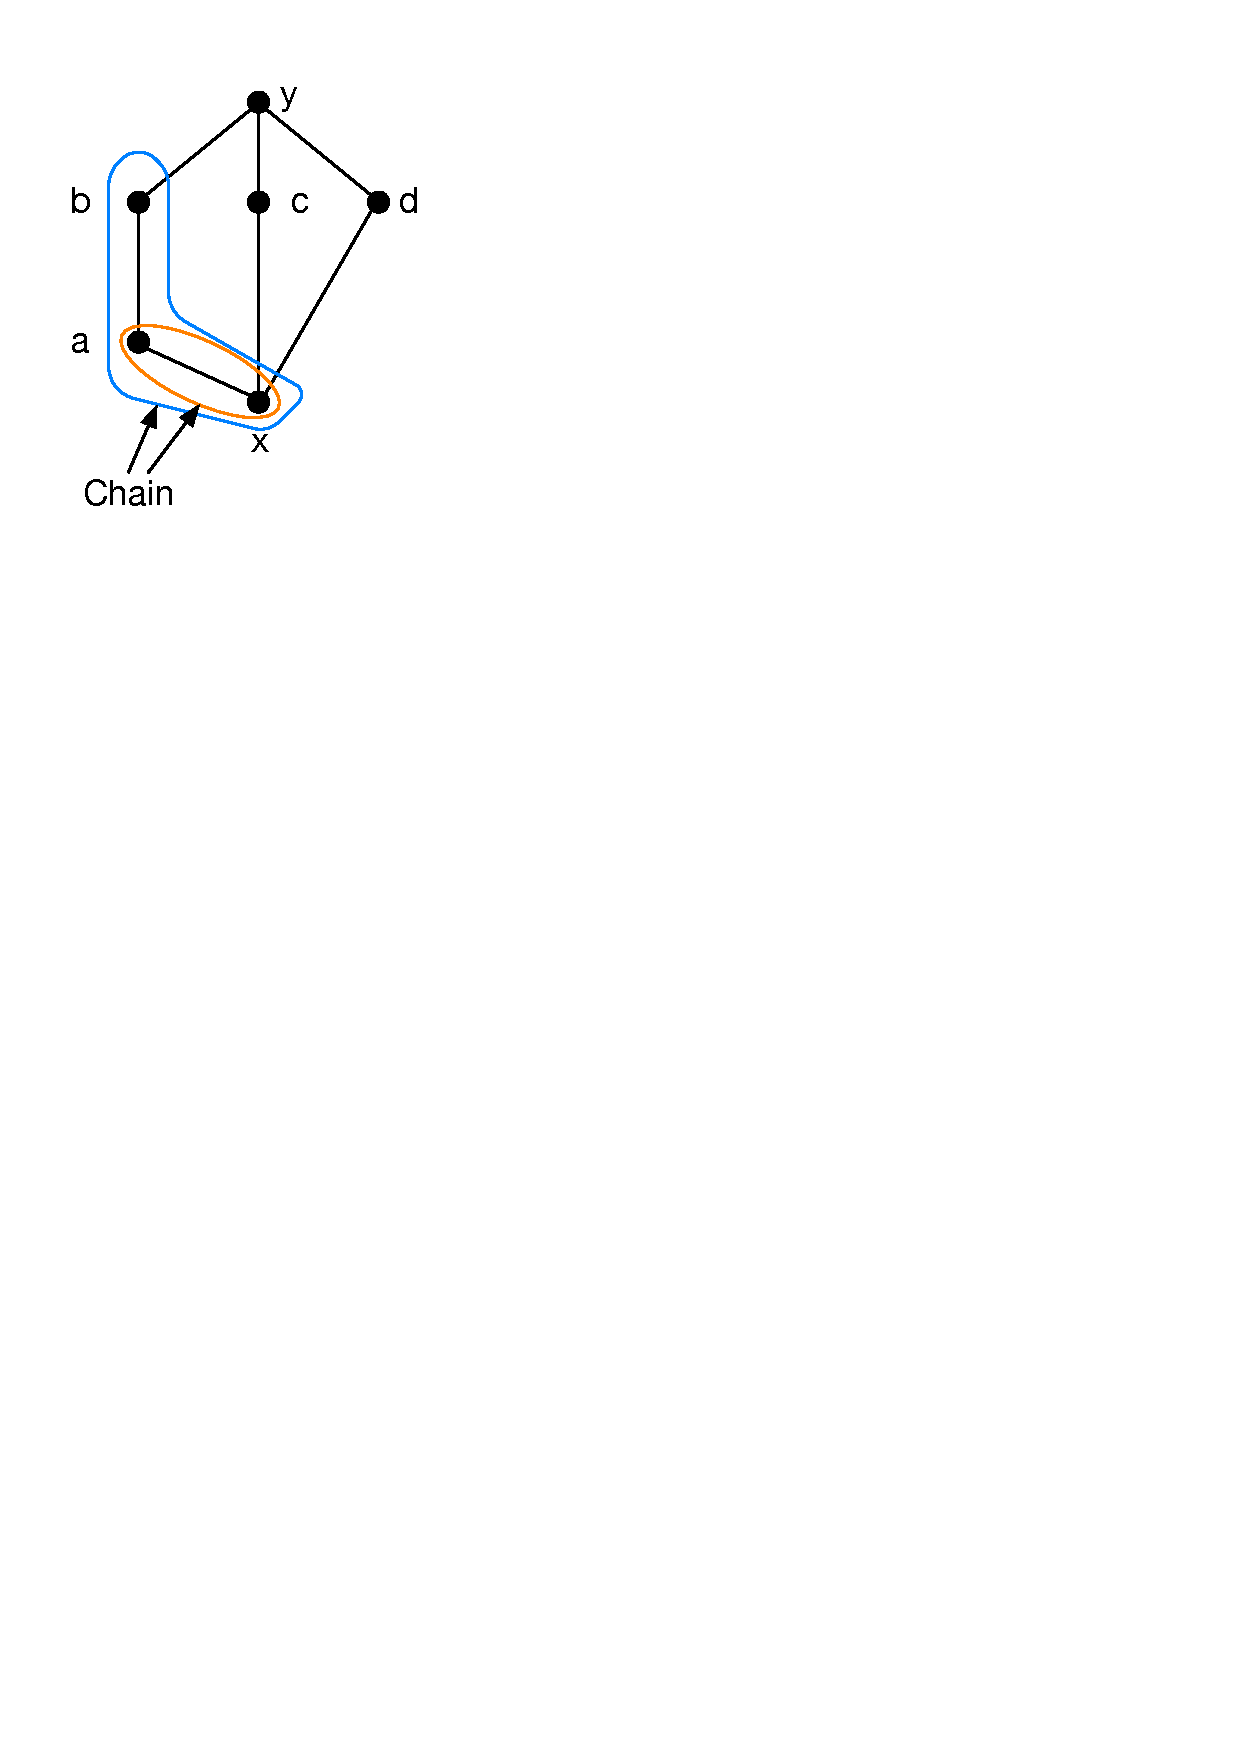
\includegraphics[width=0.3\textwidth]
      {02_higher_combinatorics/pics/LatticeMoebiusFunction}
\end{center}
\begin{align*}
    \mu(x,x) &= \mu(a,a) = \mu(b,b) = \mu(c,c) = \mu(d,d) = \mu(y,y) = 1\\
    \textcolor{orange}{\mu(x,a)} &= \mu(x,c) = \mu(x,d) = \mu(a,b) = \mu(b,y) = \mu(c,y) = \mu(d,y) = -1\\
    \textcolor{aqua}{\mu(x,b)} &= 0, \mu(a,y) = 0\\
    \mu(x,y)&:  \underbrace{\mu(x,y)}_{2}
              + \underbrace{\mu(a,y)}_{0}
              + \underbrace{\mu(b,y)}_{-1}
              + \underbrace{\mu(c,y)}_{-1}
              + \underbrace{\mu(d,y)}_{-1}
              + \underbrace{\mu(y,y)}_{1} = \delta_{x,y} = 0 \\
\end{align*}
\Theorem.
$(P_1, \leq_1), (P_2, \leq_2)$, locally finite poset, with 0-element.
And we define $(P, \leq)$ as
\[
  P = P_1 \times P_2, (x_1,x_2) \leq (y_1, y_2) :\implies x_1 \leq_1 y_1 \text{ and } x_2 \leq_2 y_2
\]

$\Rightarrow (P, \leq)$ is locally finite poset with 0-element ($=(0_1, 0_2)$) with a Möbius function $\mu: P\times P \rightarrow \mathbb{R}$
\begin{align*}
  \mu ( (x_1, x_2), (y_1,y_2)) &= \mu_1(x_1,y_1) \cdot \mu_2(x_2,y_2) \\
  (P, \leq) &= (P_1, \leq_1) \cdot (P_2, \leq_2)
\end{align*}

\textbf{Example.}
We have a Set $M = \{a_1, \ldots , a_n\}$. We claim that
\[
  (2^M, \subseteq) \cong ( \{0,1\}, \leq)^n
\]

E.g.: $n = 5: A = \{a_2,a_5\}, B= \{a_1, a_2, a_3, a_5\},\; A, B \in 2^M$
\begin{align*}
  A &\hat{=} (0,1,0,0,1) \\
  B &\hat{=} (1,1,1,0,1) \\
  A \subseteq B &\hat{=} (0,1,0,0,1) \subseteq (1,1,1,0,1) \\
\end{align*}
\[
  x \in A \rightarrow e_{x,A} = 1 \Rightarrow  e_{x,B} = 1 \implies x \in B\\
\]

Remark that: $e_{x,A} = 1 \Rightarrow e_{x,B} = 1$ is equal to $e_{x,A} \leq e_{x,B}$

\[
    ( \{0,1\}, \leq): \mu(0,0) = \mu(1,1) = 1, \mu(0,1) = -1, \mu(1,0) = 0
\]
\begin{align*}
    \mu(A,B) &= \mu(01001, 11101) = \mu(0,1) \mu(1,1) \mu(0,1) \mu(0,0) \mu(1,1) \\
    &= -1 +1 -1 +1 +1 \\
    &= 1
\end{align*}

We see that:
$A\not\subseteq B \Rightarrow \mu(A,B) = 0$,
$A\subseteq B \Rightarrow (-1)^{|B| - |A|}$.

\Theorem.
(Möbius inversion)
$(P, \leq)$ is a locally, finite poset with a 0-element.
And $\mu: P \times P \rightarrow \mathbb{R}$ the Möbius function of $(P, \leq)$.

Let for $f: P \rightarrow \mathbb{R}$ its sum function $S_f: P \rightarrow \mathbb{R}$ be given: $S_f(x) = \sum_{z \in [0,x]} f(z)$.

$\Rightarrow$: $f(x) = \sum_{z \in [0,x]} S_f(z) * \mu(z,x)$

\textbf{Example.}
$(\mathbb{N}, \leq)$, $f: \mathbb{N} \rightarrow \mathbb{R}$, $S_f(n) = \sum_{k=0}^{n} f(k)$

\[
  f(n) = \sum_{k=0}^{n} s_f(k) \mu(k,n) = s_f(n) - S_f(n-1)
\]

\Proof.
\begin{minipage}[t]{0.6\textwidth}
  \begin{align*}
      \sum_{z \in [0,x]} S_f(z) * \mu(z,x)
      &= \sum_{z \in [0,x]} \sum_{u \in [0,x]} f(u) \mu(z,x) \\
      &= \sum_{u \in [0,x]} \sum_{z \in [0,x]} f(u) \mu(z,x) \\
      &= \sum_{u \in [0,x] f(u)} \sum_{z \in [0,x]} \mu(z,x) \\
      &= \sum_{u \in [0,x] f(u)} \delta_{u,x} \\
      &= f(x)
  \end{align*}
\end{minipage}
\begin{minipage}[t]{0.3\textwidth}
  \vspace{1.2cm}
  \begin{center}
    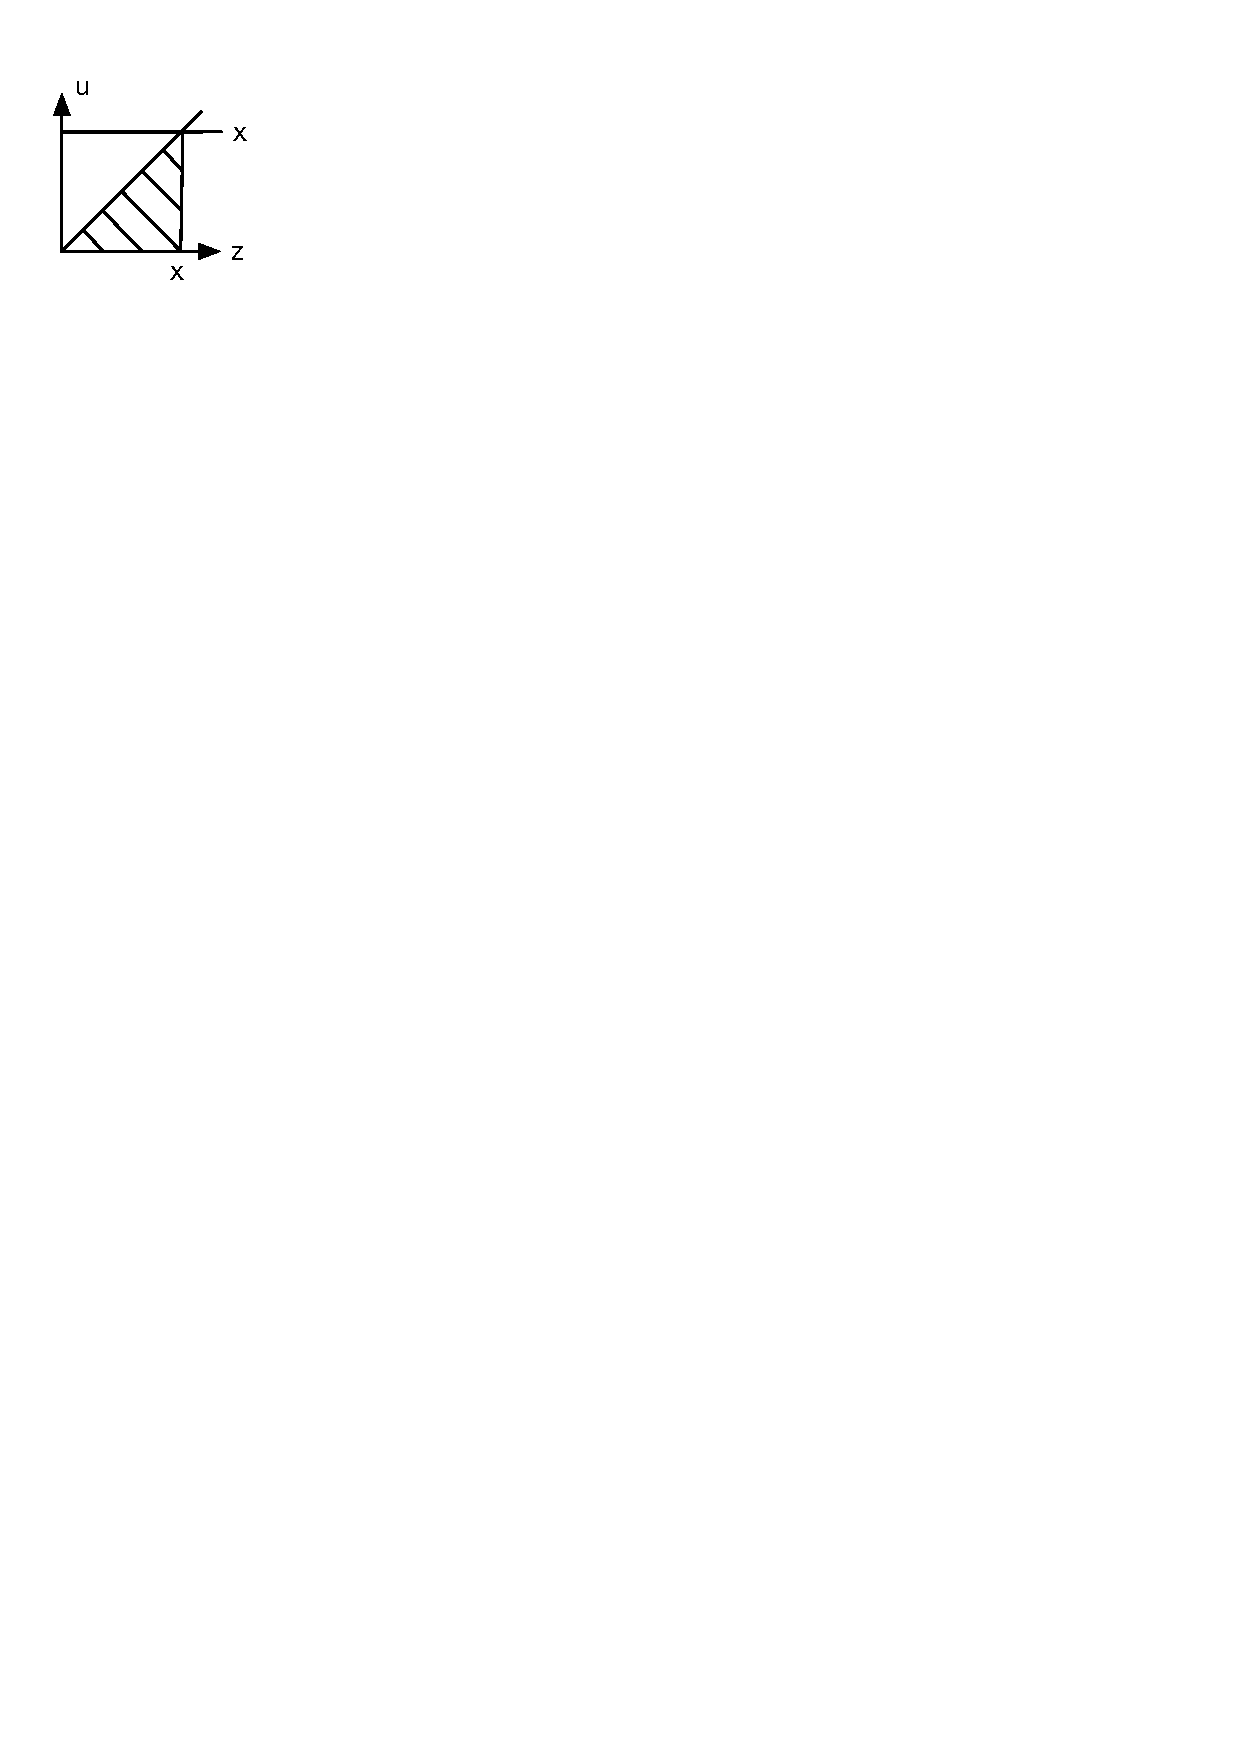
\includegraphics[width=0.8\textwidth]
      {02_higher_combinatorics/pics/MoebiusSum}
  \end{center}
\end{minipage}
